% Some commands used in this file
\newcommand{\package}{\emph}

\chapter{Introduction}
\section{Background}
The omnidirectionality of loudspeakers is not always something to aspire to but rather something that should be suppressed. This can be done by using nonlinear characteristics of air in a phenomenon known as \textit{Sound from Ultrasound}. With this principle, a highly directional steerable audio beam can be created. 

Until now, many studies have been conducted in the field of \textit{Sound from Ultrasound} and the theory of its inner workings has been mostly understood. Nevertheless, no commercially available product has yet been developed. Due to this, we decided to apply this theory gained from years of research and combine it with our ideas to create a fully functional device, the Audio-Beamformer. 

There are many potential use cases for such loudspeakers. Be it as a possibility to direct the sound of a phone call to only the person sitting right in front of a computer and mitigating the need of wearing headphones or the possibility to sit with foreign friends on the same couch and watch a movie in different languages. 
\section{Scope}
Around the task given, which can be seen in Appendix \ref{definition_of_task}, the goals of this thesis have been defined by our own.
Our first goal is to dive deep into the theory of how to generate a highly directional and steerable audio beam and get a good overview of the different technologies and ideas implemented. 
The second goal is to design a fully functioning product. For this, we set ourselves several requirements. Developing not only a working \textit{Sound from Ultrasound} loudspeaker, but also making it highly professional and easy to use. A device which is ideal for demonstration purposes.
\newpage

\section{Approach}
To achieve our goals, we started by researching different theories on creating directional sound.
We decided right from the start that the \textit{Sound from Ultrasound} principle is the way to go, mainly because of the higher directivity.
To get familiar with this kind of loudspeaker, we've searched for hardware that was ready to use. However, as there exists no commercially available product, we had to develop the hardware ourselves.
For this, we made multiple iterations of prototypes, which can be seen in Figure \ref{fig:prototype_revisions}, starting with a basic buildup on a breadboard, then soldering everything to a perfboard. After that, we designed and ordered a prototype \acrshort{pcb} and, in the end, redesigned the prototype once again and ordered the final \acrshort{pcb}.  
To test everything and quantify the obtained results, we measured everything extensively with a dedicated ultrasound microphone and conducted human expertise tests.

\begin{figure}[h!]
	\centering
	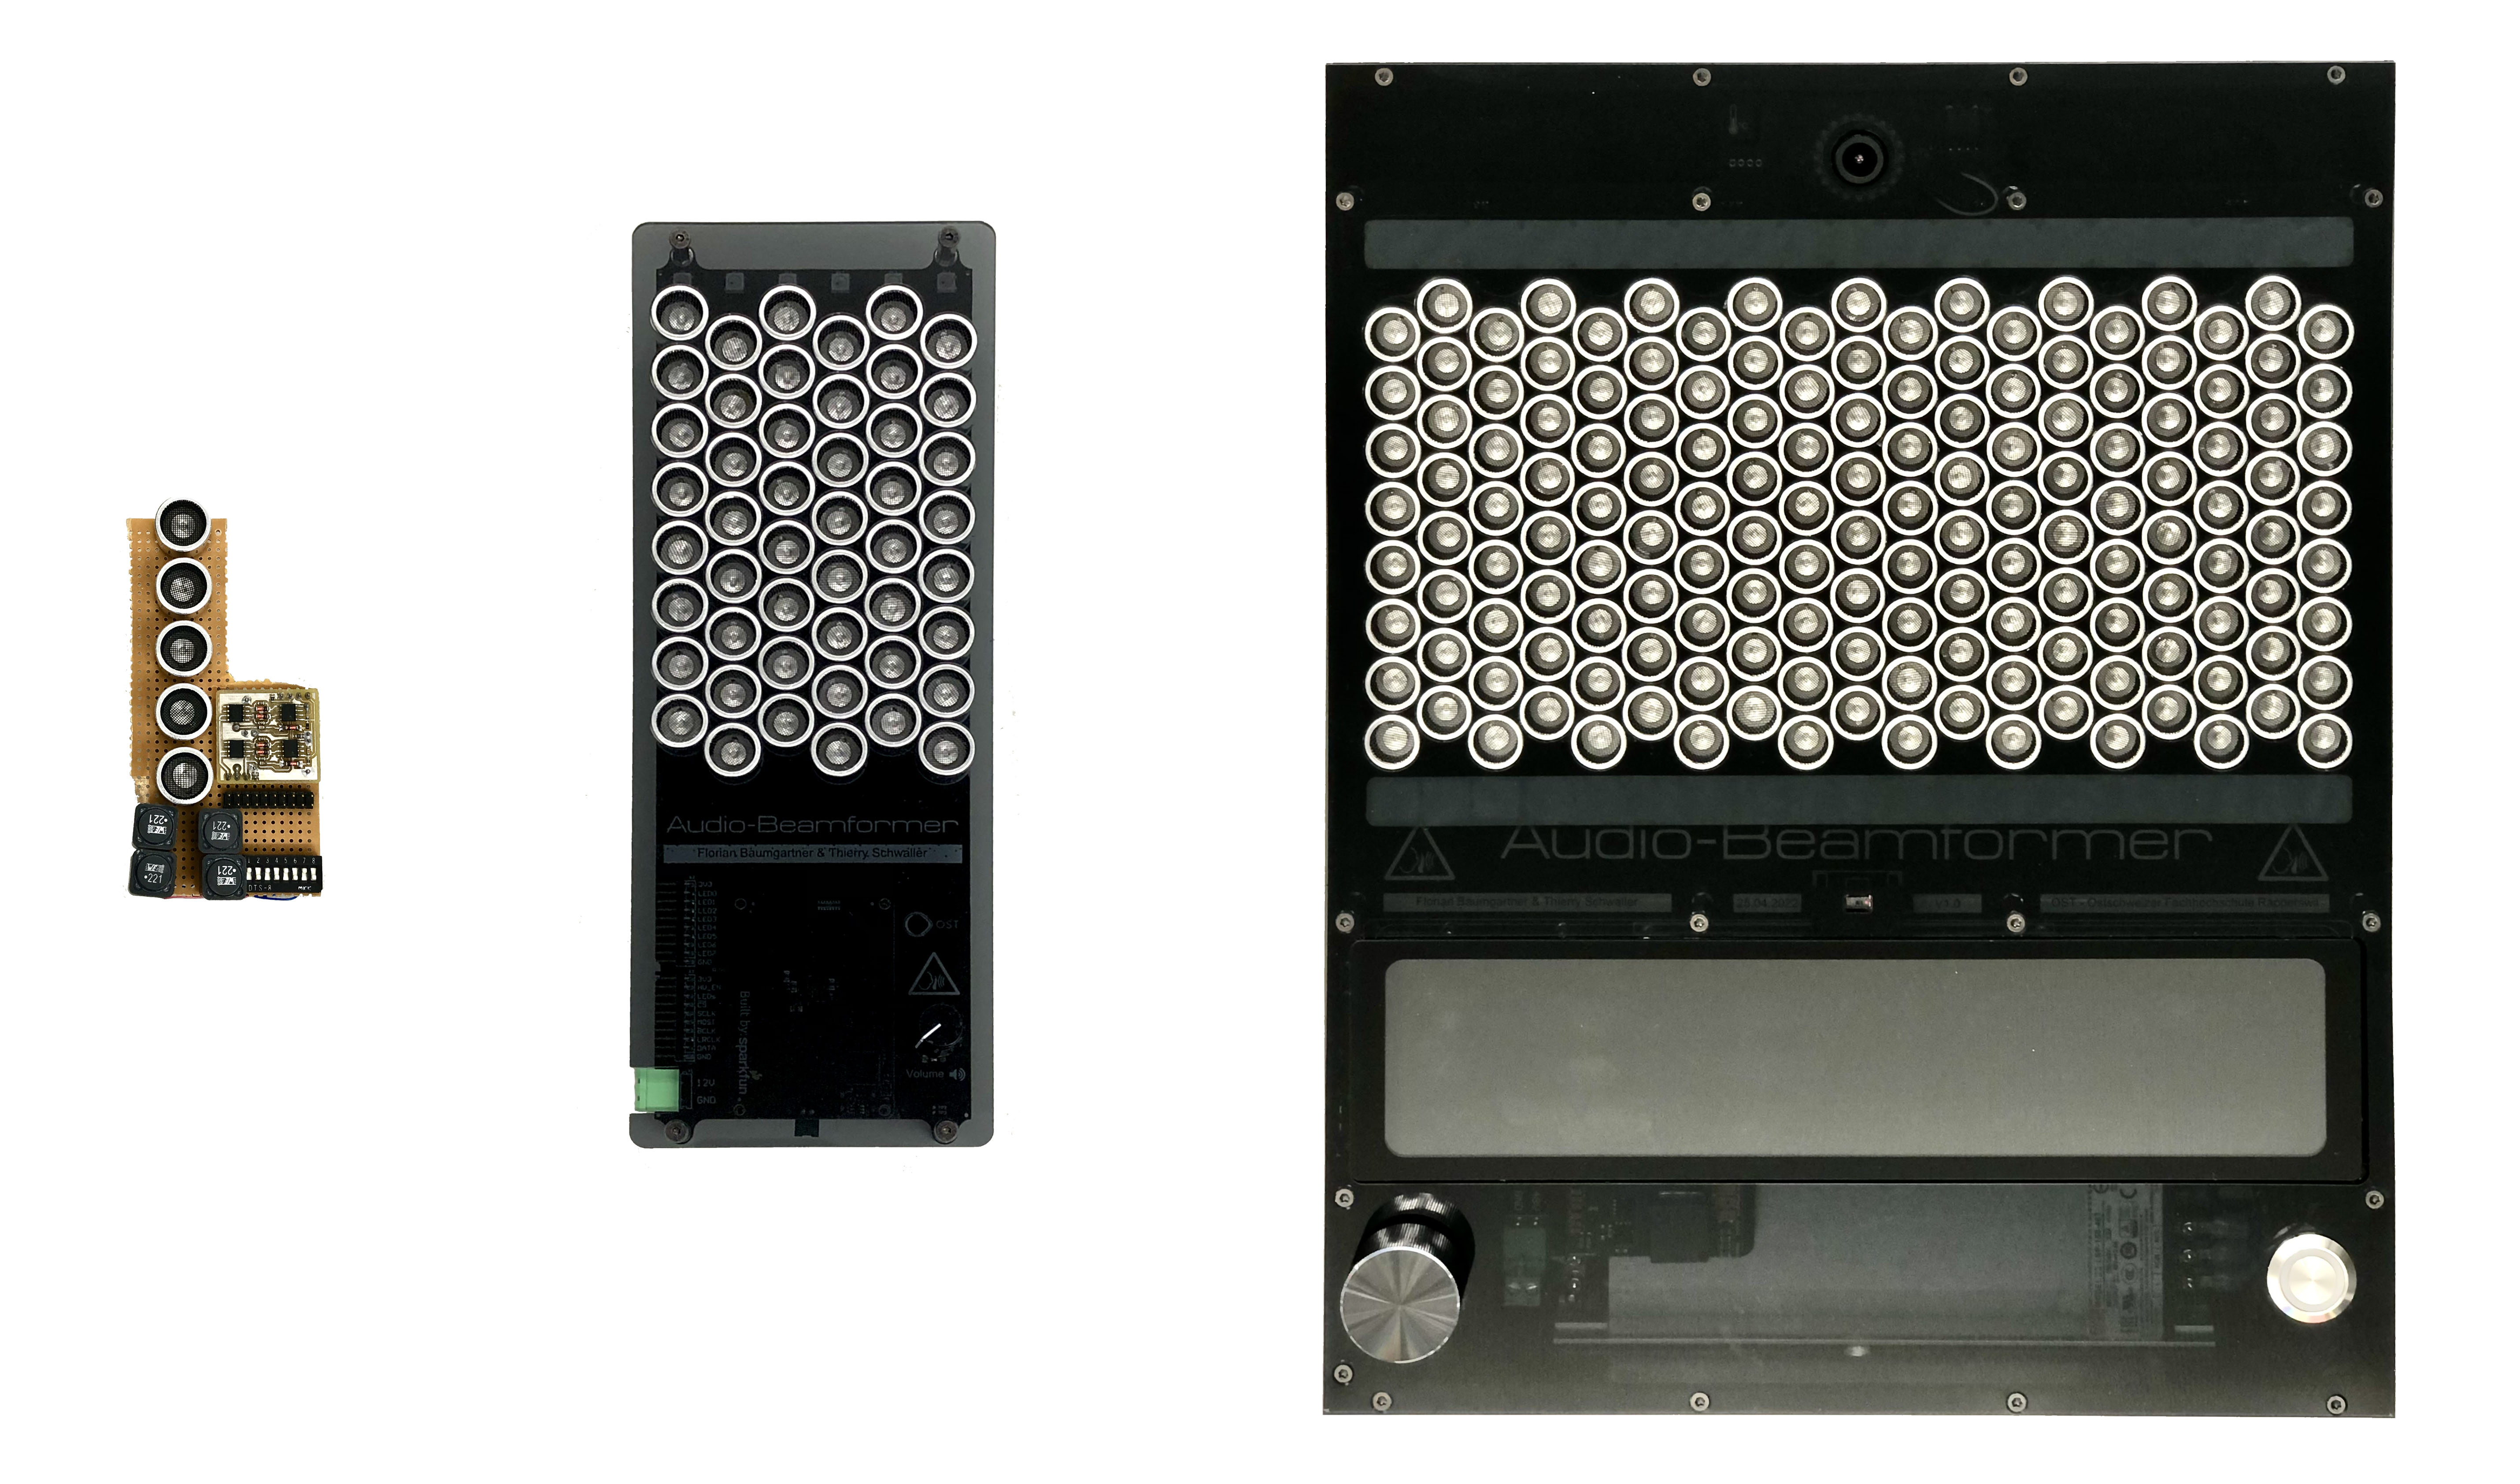
\includegraphics[width=\textwidth]{images/1_Introduction/Approach.jpg}
	\vspace{-0.4cm}
    \caption{Hardware Prototype Revisions}
    \label{fig:prototype_revisions}
\end{figure}


\section{Open Source}
Right from the start it was decided that everything about the project would be released under an open source license. Both of us are huge supporters of open source and believe it will be the future of engineering. Building upon existing libraries and code under open source licenses, allowed us to accelerate the design process. Sometimes open source is considered an act of charity, but in our case, the benefits of using it outweigh any closed source processes. All documents and files for this project can be found on our GitHub page. A short description of all the repositories can be found in the Appendix \ref{Data Archive}.
